\documentclass[conference]{IEEEtran}
% The preceding line is only needed to identify funding in the first footnote. If that is unneeded, please comment it out.
\usepackage{cite}
\usepackage{amsmath,amssymb,amsfonts}
\usepackage{algorithmic}
\usepackage{graphicx}
\usepackage{textcomp}
\usepackage{url}
\usepackage{xcolor}
\def\BibTeX{{\rm B\kern-.05em{\sc i\kern-.025em b}\kern-.08em
    T\kern-.1667em\lower.7ex\hbox{E}\kern-.125emX}}
\begin{document}

\title{Immersivaudio: audio generation based on video features.\\
{\footnotesize Group 01}
}


\author{\IEEEauthorblockN{Michele Vitale}
\IEEEauthorblockA{\textit{ist1111558}}
\and
\IEEEauthorblockN{Daniele Avolio}
\IEEEauthorblockA{\textit{ist1111559}}
\and
\IEEEauthorblockN{Teodor Chakarov}
\IEEEauthorblockA{\textit{ist1111601}}
}

\maketitle

\section{Introduction}
The topic of media generation has been exponentially growing during the last few years. Since the release of models and services based on state-of-art AI techniques, such as StableDiffusion and ChatGPT, it has been frequent to have media generative applications, with the most important part being that they can be easily accessed even by users that do not have competences and knowledge on Artificial Intelligence. 
Our proposal is a pipeline composed of different models, trained or open-wheigths, to generate audiovisive multimedia starting from a conditional video. 

\section{Problem description}
Main goal of our project is to provide a tool capable to enhance the audio track of an input video, by extracting main features such as objects, environment or tone. The tool should be easy to deploy, modular, without any particular knowledge previously required to the user, intuitive. After further research on state-of-art models, we might extend the project to also generate music. The feasibility of that, with a good quality of the outcome, will require some test at later stage, with a first part of the implementation already deployed. Further features will be implemented during the development of the project, coming out from the useful options that we might see during the development stages. 
Some researches in literature have been addressing similar problems, such as \emph{Conditional Generation of Audio from Video via Foley Analogies} \cite{du2023conditional} and \emph{Audeo: Audio generation for a silent performance video} \cite{su2020audeo}, but all of them have different goals or contexts that made them not precisely adaptable to our cause. They will still be useful in terms of architectures or proposed ideas and solutions for the problem. 

\section{Problem importance}
The problem can have a practical use in those cases in which the audio track of a video is not enjoyable, or not present at all. For instance, we can think about recordings made from drones or submarine cameras. If deployed in an accessible shape, like a very simple mobile application, the tool can be also used by visually impaired people that can get a more immersive experience from a video or from the environment surrounding them. 
Last but not least, it might result useful for content creators that need to publish their videos on platforms that have strict Copyright policies, such as YouTube. The tool could be helpful by producing some copyright-free audio track without having to rely on Copyright-free music, that might require time to be incorporated in the video track and might be already used by other creators.

\section{Architecture}
The complete architecture will be extended on four main modules, that will be connected as shown in the picture. The modules will be pluggable in a way that every single one, apart from reconstructor which is very related to the complete process, can be used as standalone parts, as long as the input shape is respected.\\
It is important to note that this is a first draft of the final architectures, so changes might apply at development stage.

\begin{figure}
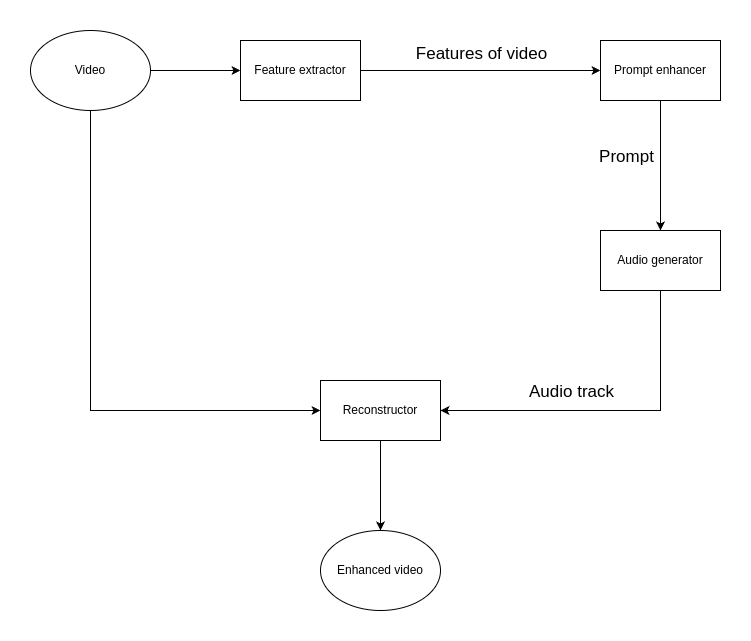
\includegraphics[width=\linewidth]{architecture.drawio.png}
\caption{Architecture schema}
\end{figure}


\subsection{Feature extraction}
The feature extraction module takes an input video, in most common video extensions, and processes it to extract relevant features such as present objects, context etc.\\
The expected output will be a list of keywords that can explain the context of the video, as well as the main subjects present. On that stage, a good starting point to be extended will be provided by repository \emph{video\_feature\_extractor} by Github user Antoine77340 \cite{vfe}, which is an extension on the video problem based on ResNet \cite{he2015deep} and ResNext models. We also plan to extend the Yolo \cite{wang2022yolov7} model and eventual other models, to have an ensemble of networks capable to extract different features by looking at the input in different perspectives.

\subsection{Prompt enhancer}
The prompt enhancer will get as input the list of features produced by the first module. The expected output will be a complete and organized prompt that will be fed to the following module. This model might be either composed by a simple string interpolated with the extracted keywords or a Large Language Model locally deployed. Components of this module will be defined with further tests on the audio generation model, to first understand what fits better for it. 
\subsection{Audio generator}
The audio generation part will be taking as input the conditional prompt, giving in output the audio track that will be combined to the video. This part will rely on audiociosioeiroeireor insert reference here, with further tests conducted in the music generation direction. AudioLDM 2\cite{liu2023audioldm} is at the moment our reference model for audio generation, since it can achieve very good results while being open source. Other models, such as MeloForm \cite{lu2022meloform}, will be further studied for the music generation part.
\subsection{Reconstructor}
This module will take both the input video and the audio track in output from the previous module, as well as eventual input parameters provided by the user. It will combine the track to the video using FFMPEG, then it return the result of the complete process to the user. 

\section{Possible features}
The basilar features that will be defined by the user will be the output format, the expected output (combined video or audio track separated), the rate from original and generated audio of a video to be mixed in the reconstruction phase.
An interesting feature that we plan to implemented is sentiment analysis and feature extraction based on the speech from an input video.
This could result in a better match between the tone of the video and the produced output track.
More features will be implemented at development time, taken out of direct observation and feedbacks on the usability of the tool.

\section*{References}

Initial references form this work are mainly composed by state-of-art models and resources that might be used during the development stage. Since the problem and the context is very dinamic and subject to tests and feedbacks, they might vary in the future adapting in accordance to the problem. 

\begin{thebibliography}{00}

    \bibitem{du2023conditional}
        Yuexi Du, Ziyang Chen, Justin Salamon, Bryan Russell, Andrew Owens,
        \emph{Conditional Generation of Audio from Video via Foley Analogies},
        \emph{arXiv preprint arXiv:2304.08490},
        2023.

    \bibitem{su2020audeo}
        Kun Su, Xiulong Liu, Eli Shlizerman,
        \emph{Audeo: Audio generation for a silent performance video},
        \emph{Advances in Neural Information Processing Systems},
        vol. 33,
        2020.


    \bibitem{vfe} antoine77340\textbackslash video\_feature\_extractor on Github \url{https://github.com/antoine77340/video_feature_extractor}. \\
    
    \bibitem{he2015deep}
        Kaiming He, Xiangyu Zhang, Shaoqing Ren, Jian Sun,
        \emph{Deep Residual Learning for Image Recognition},
        \emph{arXiv preprint arXiv:1512.03385},
        2015.

    
    \bibitem{wang2022yolov7}
        Chien-Yao Wang, Alexey Bochkovskiy, Hong-Yuan Mark Liao,
        \emph{YOLOv7: Trainable bag-of-freebies sets new state-of-the-art for real-time object detectors},
        \emph{arXiv preprint arXiv:2207.02696},
        2022. \\
    
    \bibitem{liu2023audioldm}
        Haohe Liu, Qiao Tian, Yi Yuan, Xubo Liu, Xinhao Mei, Qiuqiang Kong, Yuping Wang, Wenwu Wang, Yuxuan Wang, Mark D Plumbley,
        \emph{AudioLDM 2: Learning holistic audio generation with self-supervised pretraining},
        \emph{arXiv preprint arXiv:2308.05734},
        2023. \\

    \bibitem{lu2022meloform}
        Peiling Lu, Xu Tan, Botao Yu, Tao Qin, Sheng Zhao, Tie-Yan Liu,
        \emph{Meloform: Generating melody with musical form based on expert systems and neural networks},
        \emph{arXiv preprint arXiv:2208.14345},
        2022.
      

\end{thebibliography}
\end{document}
